\documentclass[runningheads]{llncs}

\usepackage[american]{babel}
\usepackage[english=american]{csquotes}

\usepackage[T1]{fontenc}
\usepackage{cite}
\usepackage{graphicx}
\usepackage{graphicx} % Required for inserting images
\usepackage{hyperref}
\usepackage{float}
\usepackage{xcolor}
\usepackage{amsmath} % begin{aligned}
\usepackage{amsfonts} % \mathbb{}
\usepackage{tabularx}
\usepackage[textsize=footnotesize, textwidth=40mm]{todonotes} % \todo and \todo[inline]
\presetkeys{todonotes}{fancyline}{}
\setlength{\marginparwidth}{40mm}
\usepackage{paralist}
\usepackage{enumitem}

% Enumerator for Objectives
\newlist{objectives}{enumerate}{2}
\setlist[objectives,1]{label=O\arabic*.,ref=O\arabic*}
\setlist[objectives,2]{label=(\alph*),ref=\theobjectivesi(\alph*)}

% Enumerator for Research Questions
\newlist{questions}{enumerate}{2}
\setlist[questions,1]{label=RQ\arabic*.,ref=RQ\arabic*}
\setlist[questions,2]{label=(\alph*),ref=\thequestionsi(\alph*)}


\usepackage{relsize} % for \mathlarger

% Colors tuto: https://www.overleaf.com/learn/latex/Using_colors_in_LaTeX
% \defincolor: {define new color}
%   - rgb: {r, g, b}                            [0, 1]
%   - RGB: {r, g, b}                            [0, 255]
%   - hsb: {hue, saturation, brightness}        [0, 1]
%   - HSB: {hue, saturation, brightness}        [360°, 100%, 100%]
%   - cmy: {cyan, magenta, yellow}              [0, 1]
%   - cmyk: {cyan, magenta, yellow, blacK}      [0, 1]
%   - gray: {gray}                              [0, 1] (low is dark)
%   - Gray: {Gray}                              [0, 15] (low is dark)
%   - HTML: {RRGGBB}                            6 hexa-digits
%   - wave: {wavelength}                        [363, 814] (nm)
% \colorlet: (i.e. mixing colors)
%   - \colorlet{mixedColor}{blue!10!red}        % 10% blue mixed with 90% red

\definecolor{unHighlight}{gray}{0.66}

\newcommand{\bigO}[1]{$\mathcal{O}(#1)$}

\newcommand{\mathtext}[1]{\text{#1}}
\newcommand{\indexsize}{\tiny}
\renewcommand{\index}[1]{\mathtext{\indexsize {#1}}}
\newcommand{\inmath}[1]{\relax\ifmmode #1 \else $#1$\fi}

\newcommand{\G}[1]{\inmath{G_\index{#1}}}
\newcommand{\N}[1]{\inmath{N_\index{#1}}}
\newcommand{\sk}[1]{\inmath{\text{sk}_\index{#1}}}
\newcommand{\PK}[1]{\inmath{\text{PK}_\index{#1}}}
\newcommand{\s}[1]{\inmath{s_\index{#1}}}
\renewcommand{\S}[1]{\inmath{S_\index{#1}}}

\newcommand{\sG}[2] {\relax
    \ifmmode \s{#1}\G{#2} 
    \else $\s{#1}\textcolor{unHighlight}{\G{#2}}$ 
\fi}
\newcommand{\B}[2]{\relax
    \ifmmode \mathlarger{\beta_\index{#1#2}} 
    \else $\mathlarger{\beta_\index{#1\textcolor{unHighlight}{#2}}}$ 
\fi}
\newcommand{\BB}[2]{\relax
    \ifmmode \mathlarger{\beta^\prime_\index{#1#2}} 
    \else $\mathlarger{\beta^\prime_\index{#1\textcolor{unHighlight}{#2}}}$ 
\fi}
\newcommand{\A}[1]{\inmath{\mathlarger{\mathlarger{\alpha_\index{#1}}}}}
\newcommand{\C}[1]{\inmath{\mathlarger{\mathlarger{\gamma_\index{#1}}}}}
\newcommand{\D}{\inmath{\mathlarger{\mathlarger{\mathrm{\Delta}}}}}



\newlength{\y}
\newcommand{\width}{10mm}
\newcommand{\height}{5.4mm}

\newcommand{\vgap}{
    \addtolength{\y}{-\height}
    \addtolength{\y}{-1mm}
}
\newcommand{\vGap}{
    \addtolength{\y}{-\height}
    \addtolength{\y}{-3mm}
}
%\newcommand{\hmac}{Eq. \ref{eq:integrity}}
\newcommand{\hmac}{\footnotesize $\sum$}

% Define TikZ styles
\usepackage{tikz}
\usetikzlibrary{shapes.geometric, positioning, calc, patterns, patterns.meta, backgrounds, fit, decorations.pathreplacing}
\tikzset{    
    % shape
    block/.style={draw, ultra thin, minimum width = #1*\width, minimum height = \height, inner sep = 0pt, anchor = west},
    inblock/.style={block = #1, densely dotted}, % dash pattern=on 1pt off 1pt, 
    zero_pad/.style={block = #1, fill = unHighlight, fill opacity=0.3},
    HMAC/.style={draw, ellipse, minimum width = \width, minimum height = \height, inner sep = 0pt, anchor = center},
    eq/.style={draw, circle, inner sep=1pt, fill opacity=0.2, fill=unHighlight, text opacity=1, text=black, font=\normalsize}, %font=\bfseries\large
    arrow/.style={->, shorten <= 1pt, shorten >= 2pt},
    line/.style={shorten <= 1pt, shorten >= 1pt},
    dotline/.style={dotted},
    % display
}

% Put tikz node in caption
\newcommand\eq[1][black]{ % Do not know why we need [black] to works and \eq instead of {\eq}
    \hspace{-2mm}
    \tikz[baseline=(char.base)]{
        \node [eq] (char) {#1};

    }
    \hspace{-2mm}
}

\begin{document}
	
	\title{Generating trusted sphinx packets}
	
	\author{Anonymous}
	\authorrunning{Anonymous}
	\institute{}
	
	\maketitle 
	
	\begin{abstract}
        We propose a decentralized scheme that prevent mixnets users from sending traffic that does not match the service provider of an anonymous credential.
        Our scheme is of direct use in the Nym network where users construct an anonymous credential given they receive a certificate of them paying for that service provider. 
        Our scheme prevent users from cheating by using a credential for a free service and send traffic for a paid service. 
        Our solution works even if the majority of the third parties collude. 
        Finally we evaluate the performance of our solution.
		\keywords{mixnet \and sphinx \and malicious users}
	\end{abstract}

\todo[inline]{Target: CBT Workshop on Cryptocurrencies and Blockchain
Technology; deadline: 2025-06-17; \url{https://cbtworkshop.org/}}

\section{Introduction}

Mix network, or mixnet, is an overlay network of servers (called mix nodes) that routes messages anonymously from senders
to receivers~\cite{chaum-mix,cypherpunk-remailer,piotrowska2017loopix,nym-network-whitepaper,minion-design, van2015vuvuzela,mixmaster-spec,chaum2016cmix}. Although mixnet shares similarities with Tor~\cite{onion-routing96}, they differ in two main key aspects: (i) the routing in Tor is circuit-based (meaning that all packets sent by a user follow the same path for the entire session) and in mixnets is packet-based (meaning that each packet follows a different path) and (ii) packets in Tor are forwarded immediately upon receipt by the Tor nodes while in mixnets packets are delayed for a certain amount of time $t$ in order to mitigate timing analysis attacks. These two techniques ensure that mixnets are resilient against a strong adversary who observes the entire input and outputs of the network typically called a Global Passive Adversary (GPA).
Based on Loopix~\cite{piotrowska2017loopix}, Nym Technologies is a mixnet-based system that allow users to send traffic anonymously.
Nym is a paid service where services can be integrated on the Nym network to enjoy privacy on the network level against a fee. Users of these services are then allowed to use the nym mixnet by using Nym credentials that are based on the Coconut credential~\cite{coconut}. 

For example let's say Signal is integrated with Nym, and Signal users who want their traffic to be anonymous instead of sending traffic directly to the Signal server, traffic will be first routed through the mixnet such that an adversary who observes the signal server and/or the device of the user can not correlate the sender with signal server and evetually the final recepient. Signal (service provider) can add an option for user who want to pay and issue a certified attribute to those users. Users then encode this attributes into a credential and sends it to validators. If the proof is valid, validators return partial signatures. Once the user collects a threshold number of these signatures, they aggregate them to form a valid credential and re-randomize it to ensure unlinkability from previous interactions. The user can then present this credential to a verifier to prove their right to access a service to show that the credential meets all necessary payment and authentication conditions. To prevent double-spending, the verifier checks that the credential has not already been used by consulting the blockchain and then commits the credential's serial number to the blockchain upon acceptance.

However, nothing prevents users from cheating users who might exploit valid Nym credentials to deceive the system by altering the hidden destination within the Sphinx header. For example, a user can obtain an certification from the Signal service provider, construct a valid credential and then use it to route traffic to another service provider they didn't pay for or simply not allowed (an illegal website).
Such misuse would be detected only at the final node of the mixnet preventing the user from accessing another application. 
However, prior mixnodes would have already wasted computational resources processing an invalid packet. 
This vulnerability enables Denial of Service (DoS) attack by exhausting mixnodes computational power with illegitimate packets.
\newline
In this paper we aim to address the following objectives:
\begin{itemize}
	\item Cheating users: Users's traffic is only allowed to be routed if the traffic belongs to the same service provider from the credential
	\item even if the majority of headers issuers are colluding, they do not know whcih service provider the user is communicating with.
	\item the spinx headers can not be altered.
	\item Verifiers can verify that the headers has not been altered with without revealing the service provider.
	\item Unlinkability between  sphinx packets.
\end{itemize}


In this paper we present a solution based on decentralizing the generation of Sphinx headers among trusted third parties while ensuring they learn nothing about the destination or the path. Future work include how can we use Zero-Knowledge Proofs (ZKP) to prove that the hidden destination encoded in the Sphinx header actually corresponds to an address authorized by the user’s anonymous credentials without revealing the actual destination. 
\input{Texts/2.Related_Work}
\input{Texts/3.System_Model}
\section{Our Solution - Multi-Party Computation (MPC)}\label{sec:scheme}

Our approach to ensure trust in the Sphinx header is to prevent user manipulation by decentralizing the header construction to Trusted Third Parties (TTP) through the use of Multi-Party Computaftion (MPC).
\newline

We consider TTPs as \textit{honest-but-curious}.
This means that they follow the protocol correctly but may attempt to infer additional information from the data they process.
Our design ensures that TTPs cannot infer any information about the shared secrets $ s_i $ or the involved mixnodes, even when TTPs collude (except one).
\todo{JT: In the Nym ecosystem, who are the TTPs, who operates them, what exactly are they trusted for?}
\newline

To facilitate explanation and illustration, we describe our solution in the context of a system where each packet goes through a fixed-length path consisting of three mixnodes.
However, the scheme is general and can be adapted to support arbitrary path lengths. 


\subsection{Header structure}

In our approach, each piece of header information is encoded as an elliptic curve point. 
To achieve this, the encoded string is divided into fixed-size chunks, as illustrated in Figure \ref{fig:chunked_schema}, where each chunk is a single EC point. 
For example, in the case of a path consisting of three mixnodes, the resulting header contains seven EC points: one for the destination, one for each mixnode and their integrity tag.

Therefore a method to encode and decode information to and from elliptic curve points is required. 
Specifically, we require a pseudo-random mapping between integers field and curve points group.

Traditional methods achieve this by directly mapping integers to the x-coordinates of points on the curve. 
However, this approach could leaks information by introducing bias since nearby integers result in nearby points.

To address this, we adopt Elligator, which offers stronger privacy guarantees. 
Unlike the traditional approach, Elligator produces a uniformly distributed output which is computationally indistinguishable from truly random curve points. 
This uniformity is critical in our context, where preserving anonymity and avoiding linkability are core goals. 

\subsection{Protocol description}

The overall decentralized scheme is illustrated in Figure~\ref{fig:overall_schema}.  
The client first computes a sequence of shared secrets and then splits these secrets, along with the IP addresses of the mixnodes in the path and the final destination, into $m$ shares.  
Each set of shares is sent to a different TTP, along with the necessary cryptographic element ($\ALPHA$).  
Each TTP independently computes a \textit{partial} Sphinx header using the received shares.  
The client then aggregates these partial headers to reconstruct the final header, ready for transmission through the mixnet.

\begin{figure}[H]
    \centering
    \includegraphics[width=0.8\linewidth]{Images/sphinx_ttp.png}
    \caption{[DRAFT] Overview of the decentralized scheme}
    \label{fig:overall_schema}
\end{figure}\todo{draft image}

\noindent In summary, the protocol is divided into four main steps:
\begin{itemize}
    \item \textbf{Setup}: fixes random points as generators (once but should be refreshed);
    \item \textbf{Client}: splits and shares the necessary information to TTPs;
    \item \textbf{TTP}: encrypts the routing information into a partial header;
    \item \textbf{Mixnode}: decrypts and forwards the header.
\end{itemize}


\subsubsection{Setup}

In our protocol, routing information is divided into seven chunks (see Figure \ref{fig:chunked_schema}), each one encoded into an elliptic curve point. 
These points will later be encrypted by adding a masking point of the form $ P = s G $, where $ s $ is a shared secret and $ G $ is the base generator of the curve.
However, using the same masking point $ P $ for all the seven chunks compromises the \textit{unlinkability} property
(see security note in the TTP step \ref{note:security_why_indep_generators}).

To mitigate this, we use a set of seven \textit{independent} generators $ G_j $, one for each chunk. 
By \textit{independent}, we mean that the scalar relationship between any two generators is unknown. 
Therefore no one knows the scalars $ x_j \in \mathbb{Z}_N $ such that $ G_j = x_j G $.

In principle, this setup phase can be executed only once. 
However, to preserve unlinkability, the set of generators should be refreshed periodically. 
Every entity (clients, mixnodes, and TTPs) must run the setup phase to ensure they use the same set of generators.

To achieve synchronized and deterministic generator values across the system, we derive them from a common seed. 
This seed is computed as the hash of the current timestamp, truncated to the chosen refresh interval. 
To produce distinct seeds for each generator we rehash the seed, or simply increment it since Elligator already provides a uniform (i.e. pseudo-random) integers to points mapping.
\todo[color=blue!30]{In the current implementation, instead of incrementing the seed, we rehash it for each i. However, since Elligator produces uniformly distributed outputs, incrementing may be equally secure and more efficient.}

A subtlety with Elligator is that it can map integers to points outside of the base generator's subgroup.
Thus, an extra step is required to \textit{clear the cofactor} by multiplying the resulting point by the cofactor (Curve25519's cofactor is $ 8 $).

\noindent The final formula for generating the $ j^{th} $ chunk’s generator is:
\begin{equation}
G_j = 8 \cdot H(\text{hash}(\text{timestamp}) + j), \quad \text{for } j = 1, \dots, 7
\end{equation}


\subsubsection{Client}
% 1) Define a destination
% 2) Select a random path
% 3) Select a random salt $x$ (nonce) 
% 4) Generate a chain of shared secret for the path's mixnode
% 5) Transform IP addresses (path's mixnodes and destination) into Point with Elligator and the split those point into shares.
% 6) Split the shared secrets (int) into shares.
% 7) Send sets of shares (mixnodes IPs, destination IP, shared secrets) to different TTP.
% 8) TTP will compute from those shares a partial header and send it to the client. Afterwards, the client aggregate these partial headers.
  
To send a message to a specific destination, the client first randomly chooses a path through the mixnet and generates a nonce.
Using this nonce and the public keys of each mixnode along the path, the client derives a chain of shared secret integers $ (s_1, s_2, s_3) $ as follows:
\begin{equation}
(s_1, s_2, s_3) \quad \left\{ \quad
\begin{aligned}
    \ALPHA_i    &= x_i \, G \\
    S_i         &= x_i \, \text{PK}_i \\
    s_i         &= h(S_i) \\
    r_i         &= \text{hash} ( {\ALPHA_i}_y \ \| \ {S_i}_y ) \\
    x_{i+1}     &= x_i \, r_i \quad (\text{mod}\ N)
\end{aligned}
\right.
\end{equation}
where $ x_1 $ is the client's nonce, $ \text{PK}_i $ is the public key of the $ i^{th} $ mixnode in the path, 
$ N $ is the prime order of the elliptic curve group, $ \| $ is  the concatenation operator and subscript $ y $ refers to the $ y $-coordinate of the point.
The scalar $ r_i $ acts as a pseudo-randomizer to update the secret $ x_i $ for the next hop, 
ensuring that each cryptographic element $ \ALPHA_i $ remains unlinkable across mixnodes.

The IP addresses of the mixnodes and the destination are padded with random bits
then mapped to elliptic curve points using Elligator, allowing later recovery of these addresses.
\todo[color=red!40]{Test code: to verify if the padding is still necessary or optionnal and if limited (max size N)}
Both the resulting IP points and the shared secrets are split into shares and distributed to $ m $ different TTPs. 

Each TTP then independently computes a partial header from the received shares and returns it to the client. 
The client aggregates these partial headers by performing chunkwise point additions to reconstruct the complete encrypted header.
Finally, the client sends the header along with $ \ALPHA_1 $ to the first mixnode from the path. 
\todo[color=blue!30]{Do we need to remind that the user need to encrypt his message using these shared secrets (as in original article) or is uninteresting/obvious enough ?}

\subsubsection{TTP}
% 1) Receive partial destination, path's nodes and partial shared secret
% 2) First
% 3) For each layer
Each TTP receives from the client:
\begin{itemize}
    \item a share of the destination address (EC point),
    \item a share of each mixnode address in the path (EC points),
    \item a share of each shared secrets (integers).
\end{itemize}

The TTP constructs a partial encrypted header by layering routing information in reverse path order, starting from the last mixnode, as illustrated by Figure \ref{fig:chunked_schema}.

At each layer, two new chunks are introduced: the next mixnode’s address (as an EC point) and an integrity tag.  
To preserve a fixed-length header while allowing mixnodes to reverse the operation (as in the original design), four additional \emph{filler chunks} are appended.  
These filler chunks are carefully computed such that at each layer, after applying the corresponding masking points ($s_i \ G_j$), the last two chunks cancel out and become identity point (i.e. point at infinity).  
This mechanism allows these two chunks to be safely truncated at each layer, ensuring a consistent header size while preserving reversibility for mixnodes.

To initialize the header, the TTP encrypts the destination point using the shared secret of the last mixnode and append the required filler chunks. 
Let $ \Delta $ be the partial destination point, $ s_i $ the shared secret corresponding to the $ i^\text{th} $ mixnode in the path, and $ G_j $ the $ j^\text{th} $ chunk's generator. 
The chunks for the last layer (assuming a 3-hop path) are computed as follows:
\begin{equation}
\BETA_3 \quad \left\{ \quad
\begin{aligned}
    {\BETA_3}_1 &= \Delta       + s_3 \ G_1 \\
    {\BETA_3}_2 &= - (s_2 \ G_4 + s_1 \ G_6) \\
    {\BETA_3}_3 &= - (s_2 \ G_5 + s_1 \ G_7) \\
    {\BETA_3}_4 &= - s_2 \ G_6 \\
    {\BETA_3}_5 &= - s_2 \ G_7 \\
\end{aligned}
\right.
\label{eq:last_layer}
\end{equation}

\noindent
Subsequent layers (for $ i = 2 $ and $ i = 1 $) are computed as:
\begin{equation}
\BETA_i \quad \left\{ \quad
\begin{aligned}
    {\BETA_i}_1 &= N_{i+1} + s_i \ G_1\\
    {\BETA_i}_2 &= \GAMMA_{i+1} + s_i \ G_2 \\
    {\BETA_i}_3 &= {\BETA_{i+1}}_1 + s_i \ G_3 \\
    {\BETA_i}_4 &= {\BETA_{i+1}}_2 + s_i \ G_4 \\
    {\BETA_i}_5 &= {\BETA_{i+1}}_3 + s_i \ G_5 \\
\end{aligned}
\right.
\label{eq:layer_i}
\end{equation}

\noindent
For each layer, the integrity tag is computed as:
\begin{equation}
\GAMMA_i = s_i \ G + \sum_{j=1}^{5} {\BETA_i}_j
\label{eq:integrity}
\end{equation}
Here, $ N_{i+1} $ represents the elliptic curve point corresponding to the $ (i+1)^\text{th} $ mixnode in the path.

When the first layer is finally computed, it is appended with the first mixnode’s point $ N_1 $ and the integrity tag $ \GAMMA_1 $.
Finally, the TTP returns the constructed partial header to the client.

\paragraph{\textbf{Security Note.}}\label{note:security_why_indep_generators}
To preserve unlinkability, it is essential that the generators $ (G_1, \dots, G_7) $ are \textit{independent}, meaning that their scalar relationships are unknown and cannot be derived.
If the same generator $ G' $ were used across chunks (or their scalar relationships known), an adversary could compute the chunk-wise difference between consecutive layers: $ {\BETA_i}_j - {\BETA_{i+1}}_j = s_i \ G' $.
Since the shared secret $ s_i $ remains consistent within a layer, the resulting differences would reveal a predictable pattern (uniform or preserved scalar relationships).
This consistency could allow an adversary to correlate incoming and outgoing packets at a mixnode, thereby breaking the unlinkability property.
Using independent generators for each chunk prevents such correlations and is therefore critical to the protocol's security.  

\begin{figure}[H]
    \centering
    \resizebox{0.9\linewidth}{!}{
\centering
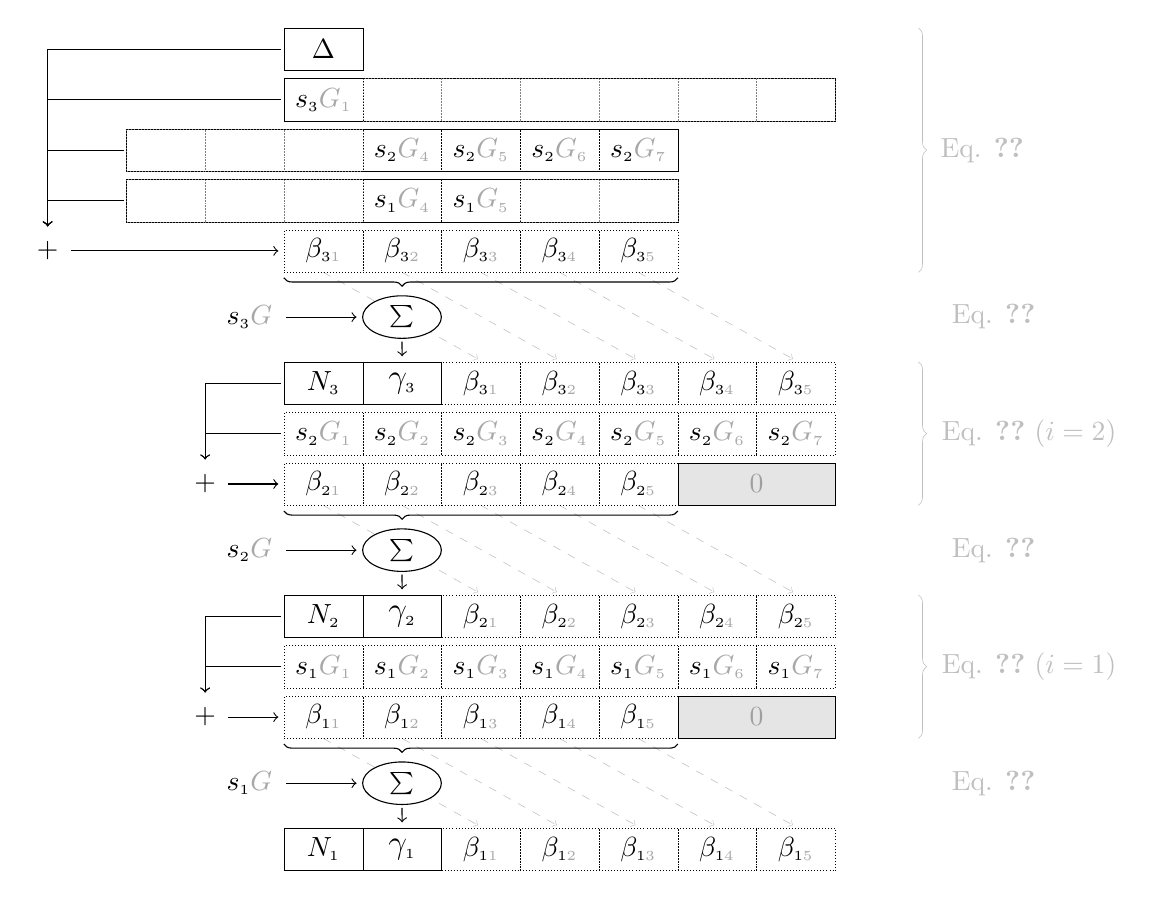
\begin{tikzpicture}
    % \tiny
    \setlength{\y}{0cm}

    \node (ip) [block=1] at (0, \y) {$\mathrm{\Delta}$};
    \vgap
    \node (s3_) [block=7] at (0, \y) {};
    \node [inblock=1] at (0, \y) {\sG{3}{1}};
    \foreach \j in {1,...,6} {
        \node [inblock=1, gray] at (\j*\width, \y) {}; 
    }
    \vgap
    \node (s2_) [block=7] at (- 2*\width, \y) {};
    \foreach \j in {0,...,2} {
        \node [inblock=1, gray] at (-\j*\width, \y) {}; 
    } 
    \foreach \j in {4,...,7} {
        \node [inblock=1] at (\j*\width - 3*\width, \y) {\sG{2}{\j}}; 
    }
    \vgap
    \node (s1_) [block=7] at (- 2*\width, \y) {};
    \foreach \j in {0,...,2} {
        \node [inblock=1, gray] at (-\j*\width, \y) {}; 
    }
    \foreach \j in {4,...,5} {
        \node [inblock=1] at (\j*\width - 3*\width, \y) {\sG{1}{\j}}; 
    }
    \foreach \j in {3,...,4} {
        \node [inblock=1, gray] at (\j*\width, \y) {}; 
    }
    \vgap 
    \foreach \j in {1,...,5} {
        \node (B3\j) [inblock=1] at (\j*\width-\width, \y) {\B{3}{\j}}; 
    }
    \node (xor3) [] at (-3*\width, \y) {\normalsize $ + $}; 
    \vGap
    \node (hmac3) [HMAC, fill=white] at (1.5*\width, \y) {\hmac};
    \vGap

    \node (n3) [block=1] at (0, \y) {\N{3}}; 
    \node (y3) [block=1] at (\width, \y) {\C{3}}; 
    \foreach \j in {1,...,5} {
        \node (b3\j) [inblock=1] at (\width + \j*\width, \y) {\B{3}{\j}}; 
    }
    \vgap
    \foreach \j in {1,...,7} {
        \node (s2\j) [inblock=1] at (\j*\width-\width, \y) {\sG{2}{\j}};
    }
    \vgap
    \foreach \j in {1,...,5} {
        \node (B2\j) [inblock=1] at (\j*\width-\width, \y) {\B{2}{\j}}; 
    }
    \node (zero2) [zero_pad=2] at (5*\width, \y) {0}; 

    \node (xor2) [] at (-\width, \y) {\normalsize $ + $}; 
    \vGap
    \node (hmac2) [HMAC, fill=white] at (1.5*\width, \y) {\hmac};
    \vGap

    \node (n2) [block=1] at (0, \y) {\N{2}}; 
    \node (y2) [block=1] at (\width, \y) {\C{2}}; 
    \foreach \j in {1,...,5} {
        \node (b2\j) [inblock=1] at (\width + \j*\width, \y) {\B{2}{\j}}; 
    }
    \vgap
    \foreach \j in {1,...,7} {
        \node (s1\j) [inblock=1] at (\j*\width-\width, \y) {\sG{1}{\j}};
    }    
    \vgap
    \foreach \j in {1,...,5} {
        \node (B1\j) [inblock=1] at (\j*\width-\width, \y) {\B{1}{\j}};
    }
    \node (zero1) [zero_pad=2]  at (5*\width, \y) {0}; 

    \node (xor1) []  at (-\width, \y) {\normalsize $ + $ }; 
    \vGap
    \node (hmac1) [HMAC, fill=white]  at (1.5*\width, \y) {\hmac};
    \vGap

    \node (n1) [block=1]  at (0, \y) {\N{1}}; 
    \node (y1) [block=1]  at (\width, \y) {\C{1}};
    \foreach \j in {1,...,5} {
        \node (b1\j) [inblock=1]  at (\width + \j*\width, \y) {\B{1}{\j}}; 
    }

    %% XOR ARROWS %%
    % 3
    \draw[arrow] (ip.west) -- ++(-3*\width, 0) -- (xor3.north);
    \draw[arrow] (s3_.west) -- ++(-3*\width, 0) -- (xor3.north);
    \draw[arrow] (s2_.west) -- ++(-\width, 0) -- (xor3.north);
    \draw[arrow] (s1_.west) -- ++(-\width, 0) -- (xor3.north);
    \draw[arrow] (xor3.east) -- (B31.west);
    % 2
    \draw[arrow] (n3.west) -- ++(-\width, 0) -- (xor2.north);
    \draw[arrow] (s21.west) -- ++(-\width, 0) -- (xor2.north);
    \draw[arrow] (xor2.east) -- (B21.west);
    % 1
    \draw[arrow] (n2.west) -- ++(-\width, 0) -- (xor1.north);
    \draw[arrow] (s11.west) -- ++(-\width, 0) -- (xor1.north);
    \draw[arrow] (xor1.east) -- (B11.west);

    %% HMAC ARROWS %%
    % 3
    \node[left=\width of hmac3] (input_hmac3) {\sG{3}{}};
    \draw[arrow] (input_hmac3) -- (hmac3.west);
    \draw [decorate, decoration={brace, amplitude=3pt, mirror, aspect=0.3, raise=2pt}] (B31.south west) -- (B35.south east);
    
    \draw[arrow] (hmac3.south) -- (y3.north);
    % 2
    \node[left=\width of hmac2] (input_hmac2) {\sG{2}{}};
    \draw[arrow] (input_hmac2) -- (hmac2.west);
    \draw [decorate, decoration={brace, amplitude=3pt, mirror, aspect=0.3, raise=2pt}] (B21.south west) -- (B25.south east);
    \draw[arrow] (hmac2.south) -- (y2.north);
    % 1
    \node[left=\width of hmac1] (input_hmac1) {\sG{1}{}};
    \draw[arrow] (input_hmac1) -- (hmac1.west);
    \draw [decorate, decoration={brace, amplitude=3pt, mirror, aspect=0.3, raise=2pt}] (B11.south west) -- (B15.south east);
    \draw[arrow] (hmac1.south) -- (y1.north);

    %% BETA ARROWS %%
    \begin{pgfonlayer}{background}
        % 3
        \foreach \j in {1,...,5} {
            \draw[->, dashed, very thin, color=lightgray] (B3\j.south) -- ([xshift=-1pt, yshift=+1pt] b3\j.north);
        }
        % 2
        \foreach \j in {1,...,5} {
            \draw[->, dashed, very thin, color=lightgray] (B2\j.south) -- ([xshift=-1pt, yshift=+1pt] b2\j.north);
        }
        % 1
        \foreach \j in {1,...,5} {
            \draw[->, dashed, very thin, color=lightgray] (B1\j.south) -- ([xshift=-1pt, yshift=+1pt] b1\j.north);
        }
    \end{pgfonlayer}

    %% TEST ANNOTATION %%
    \color{lightgray}
    \draw [decorate, very thin, decoration={brace, amplitude=3pt, raise=2*\width+30pt}]
        ([xshift=4*\width] ip.north east) -- (B35.south east) node[midway, xshift=110pt]{Eq. \ref{eq:last_layer}};
    \draw [decorate, very thin, decoration={brace, amplitude=3pt, raise=30pt}]
            (b35.north east) -- (zero2.south east) node[midway, xshift=70pt]{Eq. \ref{eq:layer_i} ($i=2$)};
    \draw [decorate, very thin, decoration={brace, amplitude=3pt, raise=30pt}]
            (b25.north east) -- (zero1.south east) node[midway, xshift=70pt]{Eq. \ref{eq:layer_i} ($i=1$)};
    % \draw [decorate, very thin, decoration={brace, amplitude=3pt, raise=10pt}]
    %         ([xshift=2*\width, yshift=-2pt] B35.south east) -- ([yshift=2pt] b35.north east) node[midway, xshift=30pt]{Eq. \ref{eq:integrity}};
    % \draw [decorate, very thin, decoration={brace, amplitude=3pt, raise=10pt}]
    %         ([xshift=2*\width, yshift=-2pt] B25.south east) -- ([yshift=2pt] b25.north east) node[midway, xshift=30pt]{Eq. \ref{eq:integrity}};
    % \draw [decorate, very thin, decoration={brace, amplitude=3pt, raise=10pt}]
    %         ([xshift=2*\width, yshift=-2pt] B15.south east) -- ([yshift=2pt] b15.north east) node[midway, xshift=30pt]{Eq. \ref{eq:integrity}};
    \node[right=6*\width+10pt of hmac3] {Eq. \ref{eq:integrity}};
    \node[right=6*\width+10pt of hmac2] {Eq. \ref{eq:integrity}};
    \node[right=6*\width+10pt of hmac1] {Eq. \ref{eq:integrity}};
\end{tikzpicture}}
    \caption{Chunkwise header encryption (TTP side)}
    \label{fig:chunked_schema}
\end{figure}


\subsubsection{Mixnode}
% 1) Extract information from the header
% 2) Recompute shared secret
% 3) Integrity check
% 4) Update encrypted information (β)
% 5) Update cryptographic element (α)


When a packet arrives at a mixnode, it begins by extracting the relevant header fields, namely the cryptographic element $ \ALPHA $ and the integrity tag $ \GAMMA $.  
The mixnode then recomputes the shared secret point $ S $ using its private key $ \text{sk} $ and the cryptographic element $ \ALPHA $:  
\begin{equation}
\begin{aligned}
    S &= \text{sk} \ \ALPHA \\
    s &= \text{Elligator}(S)\\
\end{aligned}
\label{eq:derive_secret}
\end{equation}
This point is subsequently mapped to a shared secret integer $ s $ using Elligator.
This shared secret integer is then used to verify the integrity tag: 
\begin{equation}
\GAMMA \overset{\text{?}}{=} s \ G + \sum_{j=1}^{5} \BETA_j
\label{eq:integrity_check}
\end{equation}
The integrity tag is constructed as the sum of the chunks, offset by a secret point derived from the shared secret integer. 
This ensures that only the client and intended mixnode can create, modify, or verify it.
\todo[color=red!50]{Actually, there is a vulnerability since an active adversary could randomly modify the the header and the integrity tag accordingly...}

\noindent If the integrity check passes, the mixnode pads the header by appending two \textit{identity} chunks (i.e. point at infinity) and then updates it as:
\begin{equation}
\BETA'_j = \BETA_j - s \ G_j \qquad \forall j = 1, \dots, 7
\label{eq:decrypt}
\end{equation}

The first chunk ($ \BETA'_1 $), encodes the next mixnode’s IP address. 
This point is mapped back to an integer using Elligator and the random padding is removed by keeping the last 128 bits (i.e. size of an IP address).

\noindent The second chunk ($ \BETA'_2 $) is the new integrity tag ($ \GAMMA' $) for the remaining five chunks that form the new encrypted routing information ($ \BETA' $).

To maintain unlinkability, the cryptographic element $ \ALPHA $ must be updated for the next hop. 
As in the client's step, it is computed using the $y$-coordinates of both $ \ALPHA $ and $ S $:
\begin{equation}
\ALPHA' = \text{hash}(\ALPHA_y \ \| \ S_y) \ \ALPHA
\label{eq:update_alpha}
\end{equation}
Finally, the mixnode forwards the updated header $ (\ALPHA', \GAMMA', \BETA') $ to the next node.

\begin{figure}[H]
    \centering
    \resizebox{0.9\linewidth}{!}{\centering
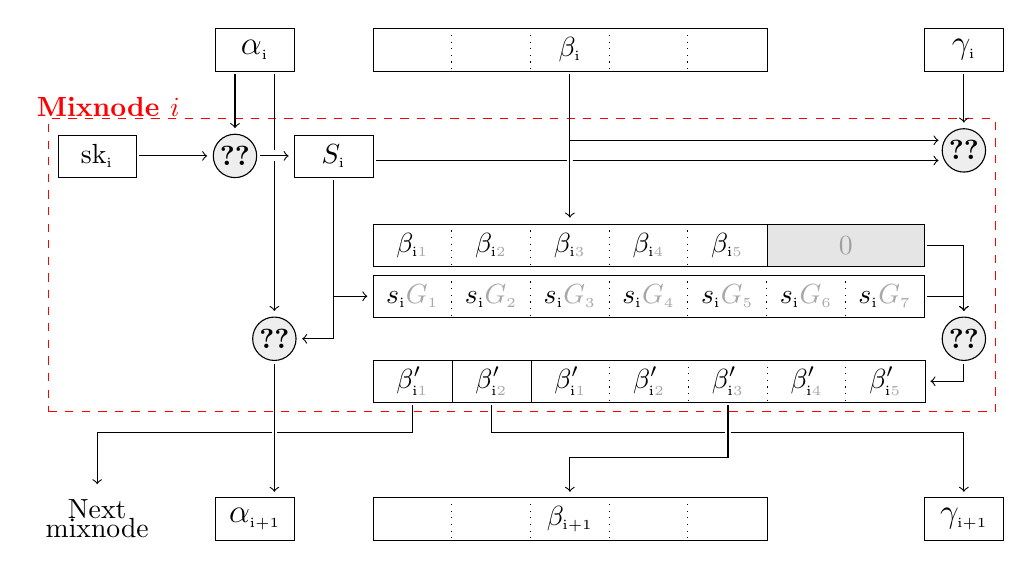
\begin{tikzpicture}
    %% INPUT
    \node (L0) at (0,0) {};
    \node (A) [block=1] at (L0) {\A{i}};
    \node (B) [block=5] at ($(A.east) + (\width, 0)$)  {\B{i}{}};
    \node (C) [block=1] at ($(B.east) + (2*\width, 0)$) {\C{i}};
    \foreach \j in {1,...,4} {
        \draw[dotline] ($(B.north west) + (\j*\width, 0)$) -- ($(B.south west) + (\j*\width, 0)$) {}; 
    }

    %% LINE 1 (shared secret, check integrity & decrypt)
    \node (L1) at ($(L0) - (0, 2.5*\height)$) {};
    \node (sk) [block=1] at ($(L1) - (2*\width, 0)$) {\sk{i}};
    \node (ss) [eq] at ($(A |- L1) - (0.25*\width, 0)$) {\ref{eq:derive_secret}};
    \node (S) [block=1] at (A.east |- L1)  {\S{i}};
    \node (check) [eq] at ($(C |- L1) + (0, 2pt)$)  {\ref{eq:integrity_check}};
 
    %% LINE 2 (decryption & blind)
    \node (L2) at ($(L1) - (0, 2.1*\height)$) {};
    \node (BB) [block=5] at (B.west |- L2) {};
    \foreach \j in {1,...,5} {
        \node (B\j) at ($(BB.west) + (\j*\width-0.5*\width, 0)$) {\B{i}{\j}};
        \ifnum \j<5
        \draw[dotline] ($(BB.north west) + (\j*\width, 0)$) -- ($(BB.south west) + (\j*\width, 0)$) {}; 
        \fi
    }
    \node (pad) [zero_pad=2] at (BB.east) {0}; 
    \node (sG) [block=7] at ($(BB.west) - (0, 1.2*\height)$) {};
    \foreach \j in {1,...,7} {
        \node (sG\j) at ($(sG.west) + (\j*\width-0.5*\width, 0)$) {\sG{i}{\j}};
        \ifnum \j<7
        \draw[dotline] ($(sG.north west) + (\j*\width, 0)$) -- ($(sG.south west) + (\j*\width, 0)$) {}; 
        \fi
    } 
    \node (N'_) [block=1] at ($(sG.west) - (0, 2*\height)$) {\BB{i}{1}};
    \node (C'_) [block=1] at (N'_.east) {\BB{i}{2}};
    \node (B'_) [block=5] at (C'_.east) {};
    \foreach \j in {1,...,5} {
        \node (B'_\j) at ($(B'_.west) + (\j*\width-0.5*\width, 0)$) {\BB{i}{\j}};
        \ifnum \j<5
        \draw[dotline] ($(B'_.north west) + (\j*\width, 0)$) -- ($(B'_.south west) + (\j*\width, 0)$) {}; 
        \fi
    }
    \node (xor) [eq] at ($(check |- sG) - (0, \height)$) {\ref{eq:decrypt}};
    \node (blind) [eq] at ($(A |- xor) + (0.25*\width, 0)$) {\ref{eq:update_alpha}};
    
    %% BOX
    \node (mixnode) [draw=red, dashed, fit=(sk) (B'_) (check)] {};
    \node[xshift=4pt, yshift=10pt] at (sk.north) {\color{red} \textbf{Mixnode $i$}};

    %% OUTPUT
    \node (L) at ($(mixnode.south) - (0, 2.5*\height)$) {};
    \node[] (N') at (sk |- L.north) {Next};
    \node[yshift=-7pt] at (sk |- L.north) {mixnode};
    \node (A') [block=1] at (A.west |- L) {\A{i+1}};
    \node (B') [block=5] at (B.west |- L)  {\B{i+1}{}};
    \node (C') [block=1] at (C.west |- L) {\C{i+1}};
    \foreach \j in {1,...,4} {
        \draw[dotline] ($(B'.north west) + (\j*\width, 0)$) -- ($(B'.south west) + (\j*\width, 0)$) {}; 
    }

    %% ARROW
    % (6) shared secret
    \draw[arrow] (A.south -| ss) -- (ss);
    \draw[arrow] (sk) -- (ss);
    \draw[arrow] (ss) -- (S);
    % (7) check
    \draw[arrow] (B.south) |- (check.+153);
    \draw[arrow] (C) -- (check);
    \draw[line] (S.east |- check.-153) -- (B.south |- check.-153); \draw[arrow] (B.south |- check.-153) -- (check.-153);
    % (8) xor
    \draw[arrow] (pad) -| (xor);
    \draw[arrow] (sG.east) -| (xor);
    \draw[arrow] (xor) |- (B'_);
    % (9) blind
    \draw[line] (A.south -| blind) -- ($(ss -| blind) + (0, 1pt)$);
    \draw[arrow] ($(ss -| blind) - (0, 1pt)$) -- (blind);
    \draw[arrow] (S) |- (blind);
    \draw[arrow] (blind) -- (blind |- A'.north);
    % xor block
    \draw[arrow] (B) -- (B.south |- B1.north);
    \draw[arrow] (S) |- (sG.west);
    % output
    \node (tmp) at ($(B'_.south) - (0, 0.7*\height)$) {};
    \draw[line] (N'_) |- (blind |- tmp); \draw[arrow] (blind |- tmp) -| (N');
    \draw[line] (C'_) |- (B'_.south |- tmp); \draw[arrow] (B'_.south |- tmp) -| (C');
    % \draw [decorate, thin, decoration={brace, mirror, amplitude=4pt, raise=1pt}] (B'_.south west) -- (B'_.south east) {};
    \draw[arrow] (B'_.south) -- ($(tmp) - (0, 9pt)$) -| (B');
\end{tikzpicture}}
    \caption{Processing sphinx header at mixnode $i$.}
    \label{fig:mixnode_decryption}
\end{figure}

\todo{Do you think it would be easier to understand/visualized the "mixnode step" with this kind of figure ?}


\section{Evaluation}\label{sec:eval}

Our prototype implementation is available on \href{https://github.com/AurelienCha/Decentralized-Sphinx}{GitHub}\footnote{\url{https://github.com/AurelienCha/Decentralized-Sphinx}}.
The implementation is written in Python 3.13 using the ECPy library for elliptic curve operations. 
ECPy is well-suited for prototyping due to its simplicity, but it is significantly slower than many EC python libraries (approximately one order of magnitude slower). 
Nevertheless, it remains one of the few Python libraries supporting Montgomery Curve25519, which is essential for our implementation.

We evaluate our system on two main axes: computational complexity and unlinkability (i.e. resistance to correlation between incoming and outgoing packets).

\subsection{Computational Complexity}

Instead of measuring raw execution time, which can vary significantly based on hardware and software environments, we focus on the number of expensive cryptographic operations. 
Table \ref{tab:operation_count} count these operations per party for $ m $ TTPs and path of length $ p $. 
To compute the total cost for sending one message, the TTP cost should be multiplied by $ m $ and the mixnode cost by $ p $.

\begin{table}[h]
    \begin{tabularx}{0.9\textwidth} { 
        l
    | >{\centering\arraybackslash}X 
    | >{\centering\arraybackslash}X 
    | >{\centering\arraybackslash}X 
    | >{\centering\arraybackslash}X  }
        & \textbf{Client} & \textbf{TTP} & \textbf{Mixnode} \\
        \hline
        \textbf{EC Multiplication}              & \bigO{p \, m} & \bigO{p^{2}} & \bigO{p} \\
        \textbf{EC Addition}                    & \bigO{p \, m} & \bigO{p^{2}} & \bigO{p} \\
        \textbf{Point $\rightarrow$ Integer}    & \bigO{p} & 0 & 2 \\
        \textbf{Integer $\rightarrow$ Point}    & \bigO{p} & 0 & 0 \\
    \end{tabularx}
    \label{tab:operation_count}
    \newline
    \caption{Number of expensive cryptographic operations per party, where $ p $ is the path length (e.g. $ p = 3 $), and $ m $ is the number of TTPs.}
\end{table}
% NOTE: Precision version
% \begin{table}
%     \begin{tabularx}{0.9\textwidth} { 
%         l
%     | >{\centering\arraybackslash}X 
%     | >{\centering\arraybackslash}X 
%     | >{\centering\arraybackslash}X 
%     | >{\centering\arraybackslash}X  }
%         & \textbf{Client} & \textbf{TTP} & \textbf{Mixnode} \\
%         \hline
%         \textbf{EC Multiplication}              & $ p (m+1) $   & $ 3 p^2 - 3 p + 2 $   & $ 2 p + 4$ \\
%         \textbf{EC Addition}                    & $ 3 p (m-1) $ & $ 5 p^2 - 7 p + 4 $   & $ 4 p $ \\
%         \textbf{Point $\rightarrow$ Integer}    & $ p $         & $ 0 $                 & $ 2 $ \\
%         \textbf{Integer $\rightarrow$ Point}    & $ p $         & $ 0 $                 & $ 0 $ \\
%     \end{tabularx}
%     \label{tab:operation_count}
%     \newline
%     \caption{\vspace*{5mm} TODO: p = path size (3) and, m is nbr of TTP (3)}
% \end{table}

Since long paths are typically unnecessary, we can approximate \bigO{p} as constant (i.e. \bigO{1}). 
A path of length $ p = 3 $ is generally sufficient to ensure strong anonymity. \todo{Aurelien: Iness do you have some source to support this ? If yes, could you cite here, thanks.}
Consequently, the overall computational burden is more sensitive to the number of TTPs $ m $ rather than the path length. 
Because our design remains secure as long as a single TTP is honest (i.e. does not collude), only a small number of TTPs may be required. 
A deeper analysis of how many TTPs are needed to ensure a desired level of trust remains an open question for future work.


\subsection{Unlinkability assessment}

Quantifying unlinkability is inherently challenging. 
However, under the assumption that uniformly random packet headers prevent adversaries from correlating incoming and outgoing packets via cryptanalysis, 
unlinkability can be approximated by assessing the statistical randomness of the headers.

We rely on the NIST SP 800-22 statistical test suite \cite{NIST-SP80022}, which includes 15 tests designed to assess the quality of random number generators. 
Each test returns a p-value representing how likely the data could be produced by a uniform source. 
If the outputs are truly random, the distribution of p-values across many samples should itself be uniform.

\todo[inline,color=blue!30]{Add a brief description of these tests (i.e. what is evaluating) -> no, too long (or for appendix)}
\todo{TODO: For the moment, only the first 4 of the 15 NIST tests have been implemented.}


For our prototype, we simulate a network of 20 mixnodes and 3 TTPs.\newline 
At each iteration:
\begin{itemize}
    \item A random destination IP and path of 3 mixnodes are selected;
    \item The client generates shares and distributes them to the three TTPs;
    \item TTPs independently compute partial headers, which are then aggregated and forwarded through the simulated mixnet.
\end{itemize}

Each run produces 4 headers (one per hop).
We perform 100 000 runs, resulting in a 400 000 x 1792 matrix (400 000 headers of 1792 bits).
Then we apply the NIST tests to each:
\begin{itemize}
    \item header independently (i.e. row-wise) to obtain p-value distributions across headers (Figure \ref{fig:sp_800-22_hist_headerwise}).
    \item bit independently (i.e. column-wise) to ensure no bias exists in specific bit positions (Figure \ref{fig:sp_800-22_hist_bitwise}).
\end{itemize}

For comparison, we conduct the same evaluation on the original Sphinx implementation by Danezis\footnote{\href{https://github.com/UCL-InfoSec/sphinx}{https://github.com/UCL-InfoSec/sphinx}}, which produces 400 000 headers of 1634 bits. 
Figures \ref{fig:sp_800-22_hist_headerwise} and \ref{fig:sp_800-22_hist_bitwise} compare header randomness of our implementation (in orange) with the original implementation (in blue).
\begin{figure}[H]
    \centering
    \includegraphics[width=0.9\linewidth]{Images/25-05-19-runwise_comparison_400000h-20n-3m-3p5.png}
    \caption{Distribution of NIST SP 800-22 p-values across 400 000 headers (headerwise evaluation).}
    \label{fig:sp_800-22_hist_headerwise}
\end{figure}
\begin{figure}[H]
    \centering
    \includegraphics[width=0.9\linewidth]{Images/25-05-19-bitwise_comparison_400000h-20n-3m-3p5.png}
    \caption{Distribution of NIST SP 800-22 p-values per bit across 400 000 headers (bitwise evaluation).}
    \label{fig:sp_800-22_hist_bitwise}
\end{figure}

Some deviations in the histograms arise from the limited size of the bitstrings (1634 or 1792 bits), which introduces quantization effects. 
In particular, the slight distortion in the first test of Figure \ref{fig:sp_800-22_hist_headerwise} reflects the granularity of possible p-values for short inputs. 
Variations in Figure \ref{fig:sp_800-22_hist_bitwise} are due to the small amount of p-values (1634 or 1792).
Increasing the histogram bin size mitigates these artifacts and confirms that the underlying distributions remain approximately uniform.

In both evaluations, the distributions of p-values are approximately uniform, which suggests that headers are statistically indistinguishable from random data, 
and therefore indicates strong linkability resistance, comparable to the original Sphinx implementation.

\subsection{Discussion}

\todo[inline]{Come back to \ref{sec:sp-objectives} objectives and explain
why they hold.}
\input{Texts/6.Conclusion}

\todo[inline]{CBT: About 15 pages till here, 16 pages in total.}

\bibliographystyle{splncs04}
\bibliography{bib}

\end{document}
